
\chapter{Protein Structure and Prediction}
\label{chap:protein_structure_and_prediction}

\section{Protein Structure}
\label{sec:protein_structure}
Twenty different \glslink{amino_acid}{amino acids}, also called residues, constitute the building blocks of proteins. Amino acids are linked in proteins by the formation of peptide bonds between amino ($NH_2$) and carboxyl ($COOH$) groups of two adjacent residues as shown in Figure \ref{fig:peptide_bond_formation}. The unique physical and chemical properties that distinguish amino acids are determined by the $R$-group. The polypeptide chain forming the protein is also referred to as backbone. In each polypeptide chain, the $N$-terminus is the end of a polypeptide chain terminated by an amino acid with a free amine group. The $C$-terminus is the end of the backbone terminated by a free carboxyl group. By convention, peptide sequences are written from the $N$-terminus (left) to the $C$-terminus (right). A review concerning protein synthesis can be found in \cite{Lengyel1969}.
\begin{figure}[tb]
	\begin{center}
		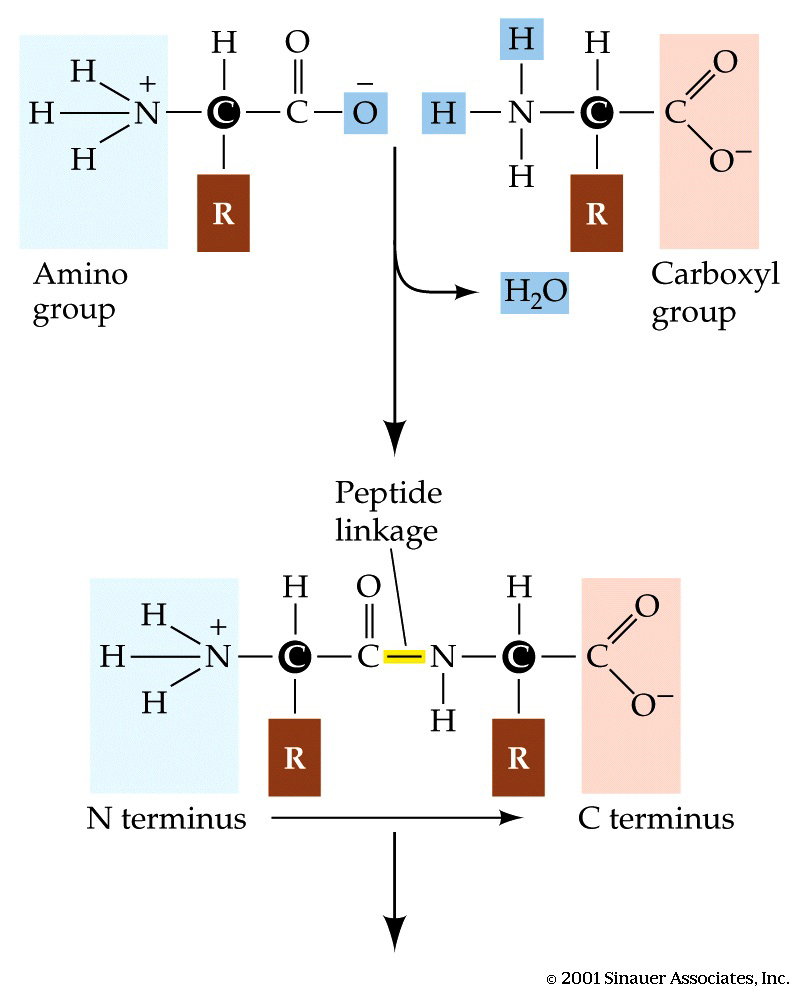
\includegraphics[scale=0.60]{peptide_bond_formation}
		\caption[Peptide bond formation]{Example of peptide bond formation. The carboxyl group ($COOH$) of the first residue binds with the amine group ($NH_2$) of the second residue, forming a peptide bond and a water molecule. The R-group is the group that distinguish an amino acid from the others.}
		\label{fig:peptide_bond_formation}
	\end{center}
\end{figure}
The backbone dihedral angles (or torsion angles) of proteins are called $\phi$ and $\psi$. The former involves the atoms $N-C_\alpha$, the latter the atoms $C_\alpha-C\ '$, as illustrated in Figure \ref{fig:dihedral_angles}. The Ramachandran plot, reported in Figure \ref{fig:ramachandran_plot}, shows all possible conformations of the angles $\phi$ and $\psi$ with the aim to analyze atom collisions by considering the van der Waals radius. Ramachandran \cite{Ramachandran1963} was the first to calculate which $\phi$ and $\psi$ angles are allowed. He modelled the permitted angles for a tripeptide, assuming the atoms were hard spheres. The allowed angles depended in part on the limiting distance chosen for interatomic contacts. The plot shows the allowed regions in red. The yellow zone describes the stable conformations, while the white zone represents collision conformations. For each residue, a specific Ramachandran plot can be defined.
There exist four levels of protein structure which refer to four distinct conceptual aspects:\\

\begin{description}
\item[Primary Structure.] The linear sequence of amino acids, encoded by the nucleotide sequence of the gene. 
\item[Secondary Structure.] The ordered array of amino acids in a protein confer regular conformational forms upon that protein. The secondary structure refers to those local structural patterns of the protein backbone.  Common elements of secondary structure are $\alpha$-helices, $\beta$-sheets and coil/loop. The $\alpha$-helix is a right or left handed coiled conformation generating a spring. The $\beta$-sheets is made of $\beta$-strands connected laterally by three or more \glslink{hydrogen_bond}{hydrogen bonds}.
\item[Tertiary Structure.] It describes the complete three-\-di\-men\-sio\-nal conformation of the protein. Figure \ref{fig:tertiary_structure_1LM8_sticks} shows an example of tertiary structure.
\item[Quaternary Structure.] It represents the arrangement of two or more different polypeptide chains forming a macromolecular complex.
\end{description}

\begin{figure}[tb]
	\begin{center}
		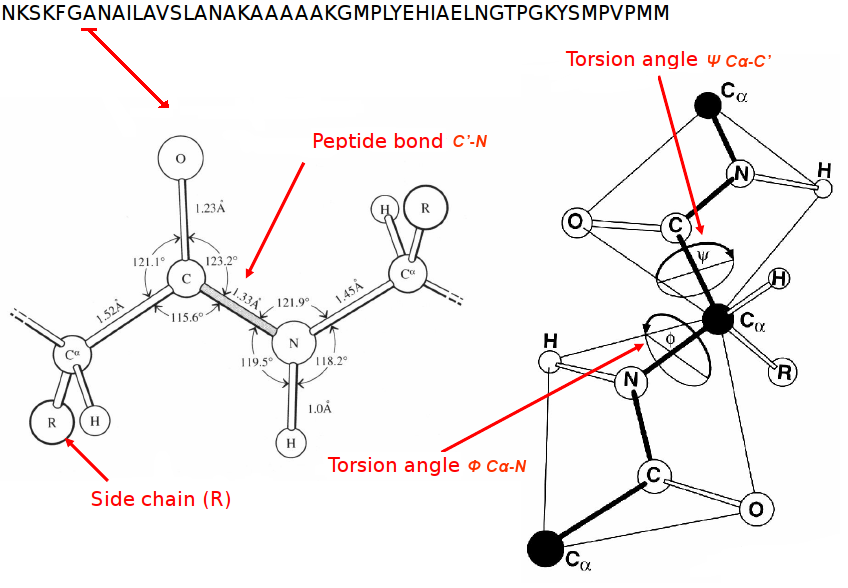
\includegraphics[scale=0.50]{dihedral_angles}
		\caption[Dihedral angles in polypeptides]{Dihedral angles in polypeptides.}		
		\label{fig:dihedral_angles}
	\end{center}
\end{figure}
\begin{figure}[tb]
	\begin{center}
		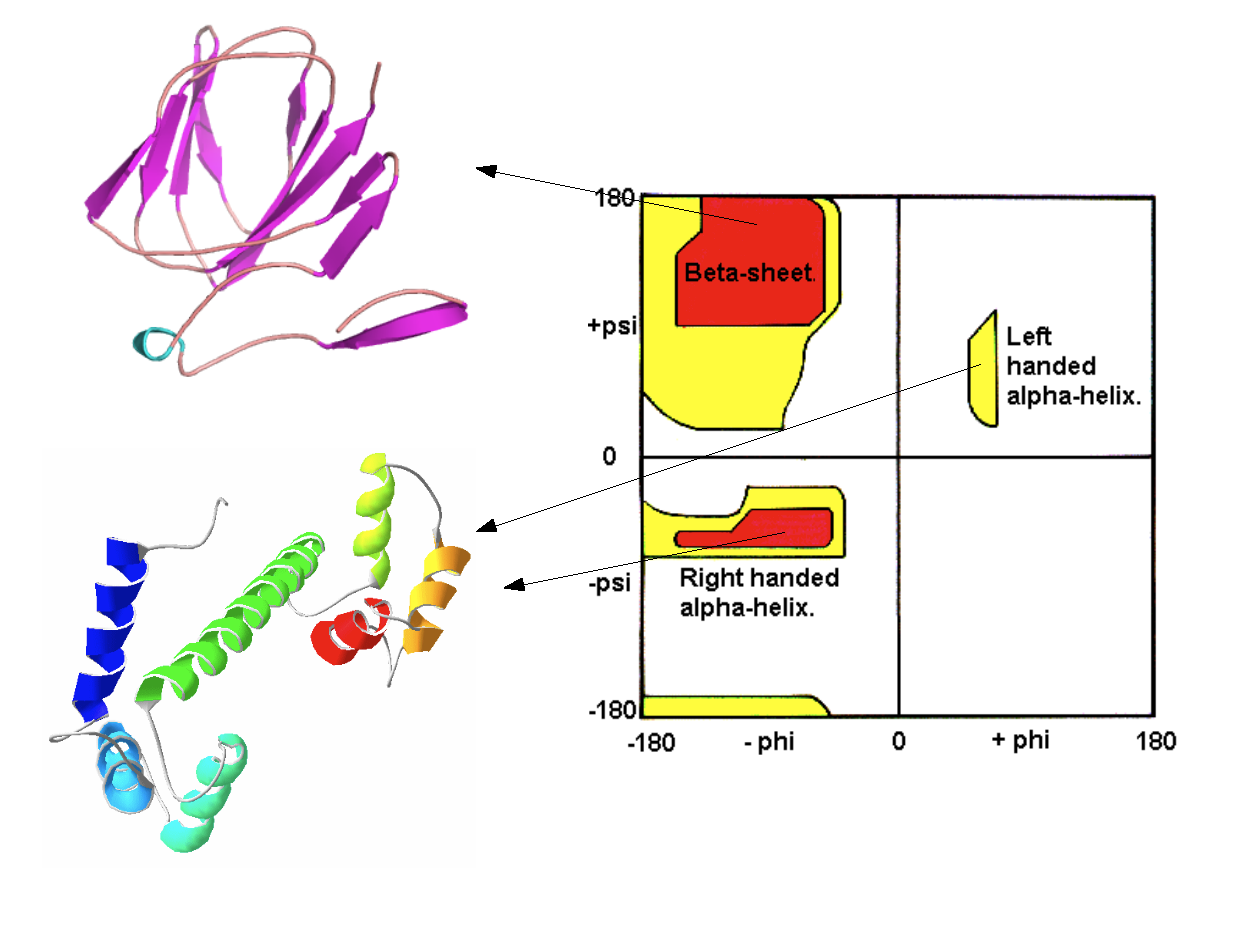
\includegraphics[scale=0.50]{ramachandran_plot}
		\caption[The Ramachandran plot]{The Ramachandran plot.}
		\label{fig:ramachandran_plot}
	\end{center}
\end{figure}
 \begin{figure}[tb]
	\begin{center}
		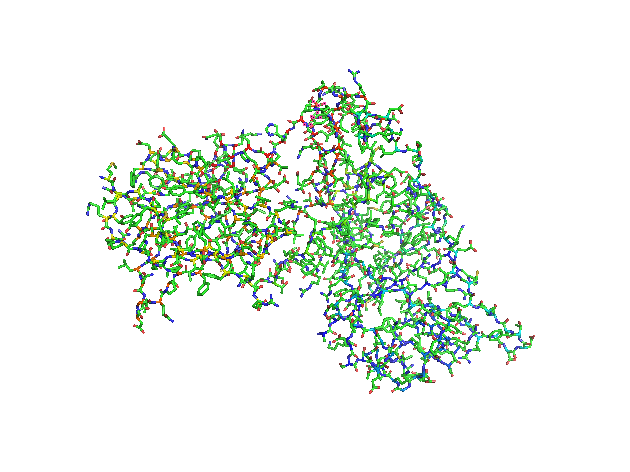
\includegraphics[scale=0.60]{1LM8_sticks}
		\caption[Tertiary structure of the protein 1LM8]{Example of the tertiary structure of the protein 1LM8.}
		\label{fig:tertiary_structure_1LM8_sticks}
	\end{center}
\end{figure}


\subsection{Sequence-Structure Relationship}
\label{subsec:sequence_structure_relationship}
Anfinsen's dogma \cite{Anfinsen1973aa} establishes that the primary sequence exclusively determines the 3-dimensional structure of a protein. Anfinsen demonstrated that the leading force for the folding process is the gradient of free energy and that the protein \glslink{native_structure}{native structure} is in its free energy minimum. Folding represents the physical process in which a polypeptide chain, such as a protein or a domain, changes state assuming its characteristic three-\-di\-men\-sio\-nal structure \cite{Lindorff-Larsen2005aa}. The folding process is still an unsolved problem \cite{Rose2006aa}. In the late 1960's, Levinthal showed that the search of all possible conformations of a polypeptide chain has exponential complexity, whereas the observed folding time is of microseconds to minutes in nature. This fact, known as Levinthal's paradox \cite{Levinthal1968aa}, demonstrates that an intensive, purely random search of the native conformation cannot succeed. Thus, he affirmed that proteins fold by following specific folding pathways.\\
Nowadays, the pathway concept based on a defined series of discrete intermediates is replaced by the concept of the energy landscape in which a multiplicity of parallel routes fall down a folding funnel. Figure \ref{fig:energy_landscape2} illustrates the funnel-like energy landscape.  The energy landscape is potentially rough due to kinetic traps and energy barriers.
\begin{figure}[tb]
	\begin{center}
		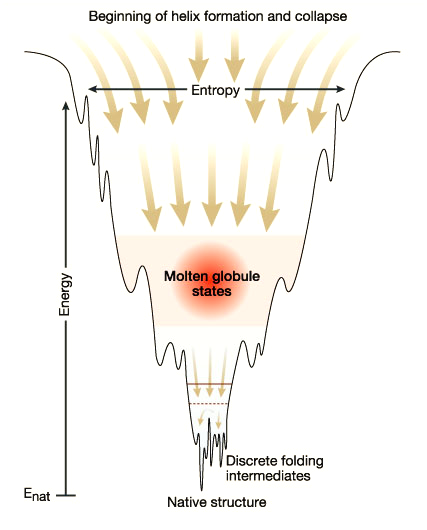
\includegraphics[scale=0.50]{energy_landscape2}
		\caption[Energy landscape for protein folding]{Energy landscape for protein folding. Protein folding does not follow a single, specific pathway, rather it follows a funnel of declining energy in which it can adopt many folding routes and still reach the native structure conformation.}
		\label{fig:energy_landscape2}
	\end{center}
\end{figure}
Often folding involves first the establishment of regular secondary and supersecondary structures, particularly $\alpha$-helices and $\beta$-sheets, and afterwards the subunits are assembled further down the folding funnel forming the known tertiary structure. The regular $\alpha$-helix and $\beta$-sheet structures fold rapidly because they are stabilized by intramolecular hydrogen bonds. The essential characteristic of folding, however, is that the amino acid sequence of each protein contains the needed information that specifies both the native structure and the pathway to reach that state. Folding is a spontaneous process independent of energy inputs. The passage to the folded state is mainly guided by hydrophobic interactions, formation of intramolecular hydrogen bonds, and van der Waals forces, and is opposed by conformational entropy \cite{Sippl1996aa}.\\
It is known that the protein function depends on the structure and this is defined by the sequence. However, prediction of protein structure from scratch solely based on physical principles currently does not achieve good results. Most current methods for protein structure prediction take into account knowledge from experimentally solved structures based on the fact that structure is more conserved than sequence.
Sequence similarity is commonly referred to as pairwise sequence identity achieved in an alignment. A pairwise alignment is a way of arranging two sequences in order to identify regions of similarity that may be a consequence of functional, structural, or evolutionary relationships between the sequences. Gaps, called also indels and denoted by ``-'', define missing residues in one or two sequences. Sequence identity describes the number of identical residues in two sequences divided by the length of the shorter sequence. After computing the sequence alignment and achieving an optimal structural superposition, the structural similarity is calculated by measuring the \gls{RMSD} between corresponding atoms of the two proteins.


\subsection{Experimental Methods}
\label{subsec:experimental_methods}
To characterize protein structures at atomic resolution, two experimental methods are usually adopted: X-ray crystallography and NMR-spectroscopy. In the Protein Data Bank (see \S~\ref{subsec:the_protein_data_bank_and_structural_genomics}), about $85\%$ of the reported protein structures are obtained by X-ray diffraction, while the remaining ones are found by NMR-spectroscopy.\\
The technique of X-ray crystallography has three basic steps. The first and often most difficult step is the production of an adequate crystal. The crystal should be sufficiently large, pure in composition and regular in structure, with no significant internal imperfections. Then, the crystal is irradiated with monochromatic X-rays, producing a diffraction pattern which is specific for the given protein structure. X-rays are waves that behave analogously to visible light on a larger scale, producing interference when scattered at the crystal. X-rays irradiating a crystal from a single direction are diffracted, which results in an interference pattern. The directions of these scattered X-rays, called reflections, depend only on the crystal lattice and not on the structure of the molecule. In this way, it is possible to collect reflections from all planes in the crystal, using a computer-guided diffractometer. The intensity of the collected reflections corresponds to the amplitudes of the molecular shape in Fourier space. Using the amplitude and the phases, the structure of the protein can be reconstructed by a Fourier transform. Unfortunately, the phase information cannot be measured by the diffractometer and additional information is needed in order to estimate the phases. A Fourier transform describes an image of the protein crystal in form of an electron density map. To place the atoms of the protein structure, the map needs to be interpreted. Because resolution for proteins is not always good enough, a further step to refine the obtained model, is required. Information about standard geometries for bond lengths and angles are used when fitting the model atoms to the electron density map. The final model is achieved by an iterative refinement of the structure. The resolution, measured in Angstrom (\AA{}), defines the accuracy of the obtained model. \\
\gls{NMR} spectroscopy is an alternative method for determining the structure of a protein in solution. The advantage with respect to X-ray crystallography is that proteins in solution are in their natural environment. However, the resolution of NMR structures is lower. The solution is exposed to a powerful magnetic field which causes the spin of the nuclei to be oriented in direction by the external field. The spin is the angular momentum of the atomic nuclei. Then, an additional magnetic field is used in order to switch the atom nuclei spin orientation. In this way the frequency, also called resonance frequency, can be measured. The resonance frequency differs for atoms depending on their chemical environment. Measuring the magnetic interaction between nuclear spins, distances of atoms close in space can be deduced. Given a sufficient number of distance constraints, these can be used to perform distance geometry calculations, with the aim to define the spatial arrangement of the polypeptide chain. NMR-spectroscopy usually produces up to $20$ or more models for a given protein, due to both the flexible character of proteins in solution and segments of the structure with few distance constraints. The more constraints are given and the closer the models become. \\
X-ray crystallography can solve structures of arbitrarily large molecules, whereas NMR-spectroscopy is restricted to relatively small molecules. X-ray crystallography defines more higher-resolution structures than NMR-spectroscopy, but is not able to capture well the molecular dynamics. Also, membrane proteins remain challenging to crystallize because they require detergents or other means to solubilize them in isolation, and these detergents often interfere with crystallization. For this kind of proteins, predictive methods are fundamental.


\subsection{The Protein Data Bank and Structural Genomics}
\label{subsec:the_protein_data_bank_and_structural_genomics}
The \gls{PDB} \cite{Berman2002aa} is a repository for the experimentally determined three-\-di\-men\-sio\-nal structural data of biological molecules, such as proteins and nucleic acids. Data submitted by biologists and biochemists from around the world are released into the public domain and can be accessed at no charge on the Web.\\
At present (March 2009) the PDB holds $52,170$ protein structures (see Table \ref{tab:pdb_current_holding_breakdown}). 
Although the number of known sequences recorded in the PDB grows exponentially, the number of newly discovered folds has decreased over the last years (see Figure \ref{fig:cewolf}). This can be due to the fact that, on one hand, some proteins, e.g. membrane proteins, are very difficult or impossible to determine with current methods; on the other hand, structural genomics initiatives have solved many of the missing folds over the last years.
Structural genomics consists in the determination of the one, two and three-\-di\-men\-sio\-nal structure of all proteins of a given organism, by experimental methods such as X-ray crystallography, NMR-spectroscopy or computational approaches \cite{Chance2004aa}. One of the major goals of the structural genomics initiative consists in high throughput protein structure determination. This allows to reduce research costs and increase the number of known structures. Targets for structural genomics are proteins with less than $30\%$ sequence identity to any structure in the PDB. Another important advantage of structural genomics is that the scientific community can immediately access to newly solved structures and relative documents.
\begin{figure}[tb]
	\begin{center}
		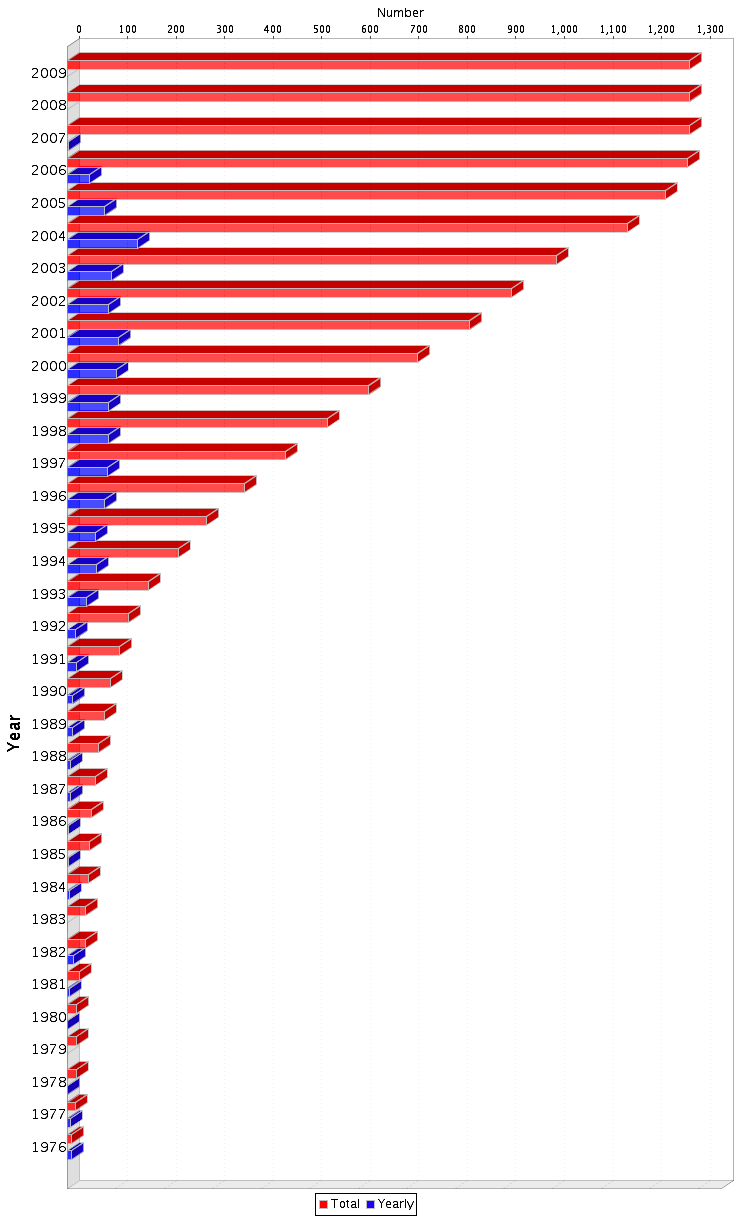
\includegraphics[width=12cm, height=15cm]{cewolf} 
		%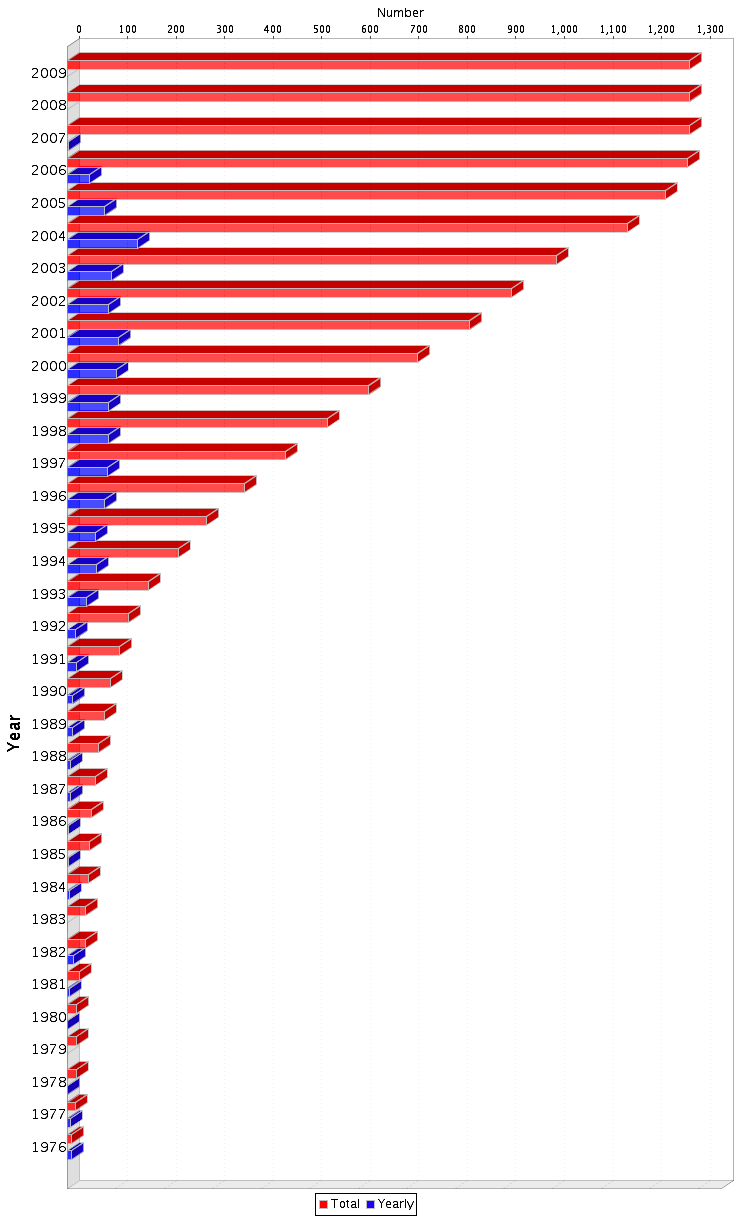
\includegraphics[scale=0.70]{cewolf}
		\caption[Growth in the number of unique folds available in the PDB, per year as define by SCOP]{Growth in the number of unique folds available in the PDB, per year as define by SCOP as of March 2009.}
		\label{fig:cewolf}
	\end{center}
\end{figure}
\begin{table}[tb]
\center
\begin{tabular}{lccc}
\toprule                % or \hline
\textbf{Exp. Method} & \textbf{Proteins} & \textbf{Nucleic Acids} & \textbf{Protein/Nucleic Acid} \\
\midrule                % or \hline
	X-ray		         &45149	&1088	&2064\\
	NMR 		         &6759	&831	&143\\
	Electron Microscopy &154		&16		&59\\
	Other			&108	&4		&4\\
	\textbf{Total} & \textbf{52170}	&\textbf{1939}	&\textbf{2270}\\
\bottomrule                % or \hline
\end{tabular}
\caption[Statistics of the PDB as of March 2009]{Statistics of the PDB as of March 2009.}
\label{tab:pdb_current_holding_breakdown}
\end{table}


\section{Protein Structure Prediction}
\label{sec:protein_structure_prediction}
The knowledge of the protein three-\-di\-men\-sio\-nal structure is important because it considerably simplifies functional annotation. Structural information is an important key from both theoretical and practical point of view. The number of known sequences (approximately $7.3$ million in UnitProt/TrEMBL\footnote{Source: \href{http://www.ebi.ac.uk/swissprot/sptr\_stats/index.html}{http://www.ebi.ac.uk/swissprot/sptr\_stats/index.html}}) is about two orders of magnitude greater than the fraction for which the structure is solved (see \S~\ref{subsec:the_protein_data_bank_and_structural_genomics}). 
Following the objective of structural genomics, new efficient and effective methods for protein structure prediction are needed, in order to close this existing gap.\\
Protein structure prediction means the prediction of tertiary structure of a protein using computational methods. The determination of the protein tertiary structure can be made in two different ways: the laws of physics and the theory of evolution. Methods that belong to the first approach are called \emph{ab initio}, while those that follow the second approach are called template-based methods.\\
\emph{Ab initio} or \emph{de novo} methods try to construct the structure of a protein based on physico-chemical properties of the amino acid chain. Theoretically, only the protein sequence is required. On the other hand, template-based methods consider structural information retrieved from known protein structures, called templates. These are used to build a model of the target sequence. From an evolutionary point of view, template-based methods are motived because structures are more conserved than sequences \cite{Chothia1986aa}. Also, they are justified by the biological reality in which there is a limited set of tertiary structural motifs to which most proteins belong \cite{Chothia1992aa}. Template-based modelling has been split into two groups: fold recognition and comparative (homology) modelling that differ on the way of template identification. The following sections deal with the different methods.\\
The choice of a good template is crucial in order to generate an accurate model for the target sequence. A good template  for a target sequence is a sequence of known structure that obtains a high similarity score when compared against the target. To highlight the importance of protein structure prediction and model quality assessment (see \ref{subsec:model_quality_assessment_programs}), it could be considered that, for instance, high to medium accuracy models, generated by homology modelling using a template with more than $30\%$ of sequence identity to the target, can be used as basis to understand interactions between residues capturing factors that arise a disease and thus be employed in drug design.


\subsection{Methods}
\label{subsec:methods}
\subsubsection{Comparative Modelling}
\label{subsubsec:comparative_modelling}
Comparative or homology modelling constructs the target structure by considering a homologous template structure. It is generally sufficient to have a sequence identity of about $30\%$ to establish a structural similarity between two proteins. This consideration is very important if related to the growth of the new experimentally solved protein structures, because it allows to increase the prediction of the structure for many known protein sequences.\\
Homology modelling refers to constructing a three-\-di\-men\-sio\-nal model of the \glslink{target}{target} protein from its amino acid sequence and an experimental three-\-di\-men\-sio\-nal structure of a related homologous protein (the template). As shown in Figure \ref{fig:comparative_modelling}, the comparative modelling framework is defined by the following steps: template identification and selection, target-template alignment, raw model building, loop modelling, side chain prediction, refinement and quality assessment. A short description of all steps is given below.\\
\begin{figure}[tb]
	\begin{center}
		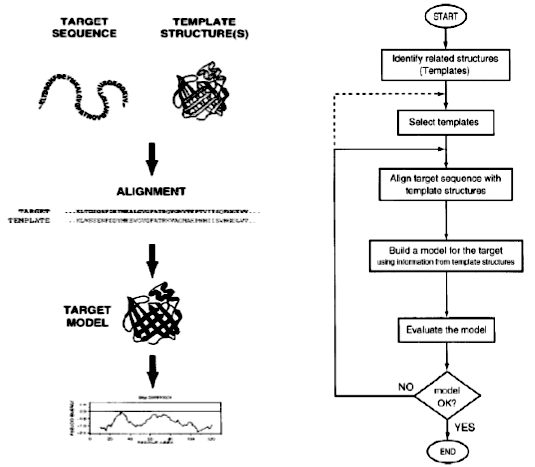
\includegraphics[scale=0.70]{comparative_modelling}
		\caption[The comparative modelling framework]{The comparative modelling framework.}
		\label{fig:comparative_modelling}
	\end{center}
\end{figure}
Comparative modelling requires at least one sequence of known three-\-di\-men\-sio\-nal structure with significant similarity to the target sequence. In order to determine if a modelling request can be carried out, the target sequence is compared with a database of sequences derived from the PDB, using programs such as FASTA \cite{Pearson1988aa} and BLAST \cite{Altschul1990aa}. The above procedure might allow the selection of several suitable templates for a given target sequence. The best template structure, that is the one with the highest sequence similarity to the target, will be used as the reference. Then, the target sequence is aligned with the template sequence. Residues which should not be used for model building, for instance those located in non-conserved loops, will be ignored during the modelling process. The next step consists in the construction of a model, which is computed by averaging the position of each atom in the target sequence, based on the location of the corresponding atoms in the template. Following the model generation, loops for which no structural information was available in the template structures are not defined and must therefore be reconstructed. Although most of the known available three-\-di\-men\-sio\-nal structures share no overall similarity with the template, there may be similarities in the loop regions, and these can be inserted as loop structure in the new protein model. For many of the protein side chains there is no structural information available in the templates. These therefore cannot be built during the model generation and must be added later. The number of side chains that need to be built is established by the degree of sequence identity between target and template sequences. To this end, a table of the most probable rotamers for each amino acid side chain depending on their backbone conformation is used. The most favoured rotamer is added to the model. By energy minimization with force fields (see Appendix \ref{appendix:force_fields_statistical_potentials}), bond geometry and removal of unfavorable non-bonded contacts can be refined. It is necessary to keep the number of minimization steps to a minimum in order to avoid a distorted model.\\
The quality of the homology modelling is dependent on the quality of the sequence alignment and template structure \cite{Fasnacht2007aa, Lee2007aa}. The approach can be complicated by the presence of alignment gaps that indicate a structural region present in the target but not in the template, and by structure gaps in the template that arise from poor resolution in the experimental method (see \S~\ref{subsec:experimental_methods}) used to solve the structure. It is known that model quality declines with decreasing sequence identity; a typical model has $\approx 1.5$ \AA{} RMSD between the matched $C_{\alpha}$ atoms at $70\%$ sequence identity but only $\approx 3$ \AA{} RMSD at $25\%$ sequence identity. However, the errors are significantly higher in the loop regions, where the amino acid sequences of the target and template proteins may be completely different. Regions of the model that were constructed without a template, typically by loop modelling, are generally much less accurate than the rest of the model. Errors in side chain prediction also increase with decreasing identity \cite{Eramian2006aa}.\\

\subsubsection{Fold Recognition}
\label{subsubsec:fold_recognition}
The original distinction between homology modelling and fold recognition consisted in the difficulty to identify and select a suitable template. Fold recognition requires more sophisticated techniques in order to obtain an adequate template. In other words, homology modeling is for easy targets and fold recognition is for hard ones. At present, fold recognition-like approaches are commonly used in protein structure prediction and also in \emph{ab initio} methods (e.g. \emph{novel fold} methods).\\
The fold recognition assumptions are that the protein structure is much more evolutionarily conserved than sequence \cite{Chothia1986aa} and that the number of adopted protein folds is limited \cite{Chothia1992aa}. In particular, two proteins could fold in the same structure even if the sequence similarity is either very low or non-existent.
At CASP (see \S~\ref{subsec:casp}), assessors distinguished fold recognition targets into homologous and analogous folds. Homologues are evolutionarily related sequences that derive from a common ancestor. Analogues are sequences for which it is unknown if an evolutionary relationship exists. Modern sequence alignment methods such as PSI-BLAST \cite{Altschul1997aa}, demonstrated that some proteins which have been previously considered as analogues, are instead homologues.\\
Two different categories exist in fold recognition: threading and profile methods. The original aim of the development of threading methods was to find out folds for analogous targets. The name ``threading'' was suggested from the ideal threading of a target sequence in a fold library by identifying the protein fold that best fits the target. The local amino acid conformation and the structural information are taken into account in order to evaluate each residue. In more detail, to define the residue local conformation the common approaches are based on contact potentials \cite{Jones1992aa, Sippl1990aa}. On the other hand, to represent the structural environment of residues, three-\-di\-men\-sio\-nal profiles  are developed \cite{Bowie1991aa}. To generate an alignment between the target and template, techniques based on dynamic programming algorithms are commonly adopted. The effect of this alignment is the consequent changing of the structural environment. Contact potentials \cite{Pollastri2001aa} and other statistical potentials \cite{Jernigan1996aa} are often used to evaluate the candidate models for the target sequence. More details dealing with statistical potential are reported in Appendix \ref{appendix:force_fields_statistical_potentials}. Such potentials are also adopted in other bioinformatics fields such as model quality assessment (see \S~\ref{subsec:model_quality_assessment_programs}).\\
The second class of fold recognition methods, contemplates profile or mapping programs. These aim to identify templates that are weak sequence homologues to the target sequence. Profile methods make the assumption that conserved sequence motifs are more relevant than the variable parts of a sequence when performing an alignment. A profile describes conserved regions of a family of homologous proteins. Thus, methods based on profile-sequence alignment have been developed. The best known method of this category is PSI-BLAST. Recently, with the same intent, a new generation of methods based on profile-profile alignment \cite{Sadreyev2003aa} have been designed and implemented. These utilize Hidden Markov Models in order to increase both the sensitivity in capturing weak evolutionary relationships and accuracy with respect to current methods. In more detail, a profile of the query sequence is computed and then aligned to the profile of every template protein by using a specific scoring function. The need to have a profile for every sequence recorded in the database has limited the application of these new methods due to high computational costs. \\
Another improvement in method accuracy can be achieved by considering information from predicted secondary structure and/or predicted solvent accessibility \cite{Jones1999aa, Pettitt2005aa}. This additive information can be incorporated directly in sequence profiles or used as features in threading-based approaches.


\subsubsection{Ab Initio and Novel Fold}
\label{subsubsec:ab_initio_and_novel_fold}
A completely different approach to the protein structure prediction is based on so called \emph{Ab initio} or \emph{de novo} methods. The idea behind \emph{ab initio} methods is to predict the native structure of a protein by the simulation of the real folding process. In order to do this, molecular mechanics force-fields and molecular dynamics simulations are commonly used. These kinds of methods require a lot of computational time and produce imprecise and often incomplete models.\\
In the last years, the pure \emph{ab initio} approach, based on the physical principles solely has been put aside by many research teams that have preferred to also utilize available structural information. This new approach has allowed to improve the quality of predicted models. Structural information can be obtained through fragments extracted from known protein structures (this category of \emph{ab initio} methods is called \emph{novel fold} methods). \emph{Ab initio} structure prediction suffers for two problems: the huge amount of admissible generated conformations and the inaccuracies of the scoring functions. With the intent to reduce the number of produced models and thus overcome the first problem, reduced representations of the conformations have been adopted. ROSETTA \cite{Bonneau2002aa, Simons1997aa} is a successful method that assembles structures from short protein fragments (\emph{novel fold} methods). Other prominent methods consider lattice-based simulations \cite{Ortiz1999aa, Zhang2003aa}. One of the best recent methods is TASSER (Threading/ASSEmbly/Refinement) \cite{Zhang2005aa} which builds the model from structural fragments of templates selected using a threading technique, while it constructs the other unknown protein parts by adopting a lattice-based approach.


\subsection{CASP}
\label{subsec:casp}
\glslink{CASP}{CASP}\footnote{\href{http://predictioncenter.org/}{http://predictioncenter.org/}}, which stands for Critical Assessment of Techniques for Protein Structure Prediction, is a community-wide experiment for protein structure prediction. It aims to establish the current state of the art, identifying what progress has been made, and highlighting where future effort may be most productively focused. It takes place every two years during which the predictors from different research teams receive a set of protein sequences for which the structure is to be experimentally solved. During the prediction season, about $3$ months, predictors do not know the native structures. After this period, the quality of the submitted models is assessed and results are presented at the CASP conference \cite{Zemla2001aa}.\\
Over the years, the number of prediction \glslink{target}{targets} has increased from $33$ in $1994$ (CASP-1) to $117$ in December $2008$ (CASP-8). At the beginning, targets were classified in comparative modelling, fold recognition and new folds, by considering the method used. Since the seventh round of CASP, the categories have been reformulated in free modelling and template-based modelling. The latter category includes a subset of tertiary structure models in which the backbone is sufficiently accurate so that the details of the side chains, loops, and active sites can be meaningfully assessed. This subset of structures, called high accuracy models, is selected from the best models received during the prediction season.\\
CASP-8 is particularly address the following questions:
\begin{enumerate}
\item Are the models produced similar to the corresponding experimental structure?
\item Is the mapping of the target sequence onto the proposed structure (i.e. the alignment) correct?
\item Have similar structures that a model can be based on been identified?
\item Are comparative models more accurate than can be obtained by simply copying the best template?
\item Has there been progress from the earlier CASPs?
\item What methods are most effective?
\item Where can future effort be most productively focused?
\end{enumerate}
At the last CASP experiment (CASP-8), $234$ research groups have participated. Of these, $45$ model quality assessment programs have been presented. The total number of models proposed has been $29,066$.

\subsection{Model Quality Assessment Programs}
\label{subsec:model_quality_assessment_programs}
Both \emph{ab initio} methods and recent template-based approaches, produce a lot of possible models. \gls{MQAP} is a new category, introduced in CASP-7, with the aim to assess the quality of predicted models \cite{Cozzetto2007aa}. MQAP can be distinguished in two classes: local and global assessment. The former is intented to establish the inner quality of a structure by predicting the RMSD distances between residues of the considered target structure and the corresponding residues of the native one \cite{DeRonne2008aa, Fasnacht2007aa}. The latter defines a global quality for each predicted model in order to rank them by quality. This evaluation is of interest both for Homology Modeling targets, where it is important to select the best model among a set of many good, \emph{correct} ones as well as for the other targets, where the set may contain many incorrect models. A drawback of global assessment is that it does not recognize correct and incorrect regions that might exist in a protein model. For this reason, local assessment exists. This thesis will concentrate on the global assessment subclass. An MQAP is a computer program that receives as input a three-\-di\-men\-sio\-nal predicted model in PDB format and produces as output a real number representing the quality of the model without using the native structure information. There are also two main MQAP method types. Single-model methods use features computed from the structure, while clustering-based methods use the similarity to other models. Section \S~\ref{sec:state_of_the_art} describes the main MQAP methods.\\


\section{State of the Art}
\label{sec:state_of_the_art}

\subsection{Evaluation of Global Quality}
\label{subsec:evaluation_of_global_quality}
At the time of writing, standard evaluation measures of model global correctness are \gls{GDT} \cite{Zemla2001aa}, TMscore \cite{Zhang2004}, MaxSub\cite{Siew2000}, Pearson and Spearman correlation coefficients. GDT\_TS uses four thresholds, 1, 2, 4 and 8 \AA{} and computes the average across the four thresholds. TMscore takes into account that smaller proteins tend to have lower RMSD, and varies the distance threshold according to the size of the protein. MaxSub considers a substructure to be well-predicted if distances between equivalent residues in the substructure after superposition are below a constant threshold of 3.5 \AA{}. Other model quality measures are reported in \cite{Cristobal2001aa}.

\subsection{Scoring functions}
\label{subsec:scoring_functions}
Scoring functions has been used in model quality assessment to discriminate between high quality and misfolded ones. An ideal scoring function should have perfect correlation with the quality of the structural model, which is measured by the closeness of the model to the native structure. Scoring functions rely on the thermodynamic hypothesis stating that the native state of a protein lies in the free energy minimum under physiological conditions (see \S~\ref{subsec:sequence_structure_relationship}) \cite{Lazaridis2000aa}. They can be derived by one of three following approaches: 
\begin{description}
\item[Physical potentials.] A physical potential computes the energy of a structure by modelling the interactions between different components of the protein or between the protein and the solvent based on physical laws. The parametrization is performed either by fitting experimental data or based on quantum chemical calculations \cite{Fogolari2003aa, Lazaridis1999aa}.
\item[Probability distribution based potentials.] A probability dis\-tri\-bu\-tion-\-based potential extracts the energy parameters from probability distributions of known native structures \cite{Bahar1997aa, Sippl1990aa}. Statistical potentials are based on the Boltzmann equation, which relates frequencies of observed structural features to their energy.
\item[Machine learning-based scores.] Machine learning-based scores are computed by machine learning techniques such as \glslink{ANN}{artificial neural networks (ANN)} \cite{Mereghetti2008aa} and \glslink{SVM}{support vector machines (SVM)} \cite{Qiu2008} in order to learn how to combine multiple features, from a training set including structures of different quality. 
\end{description}
More details on statistical potentials and force fields are given in Appendix \ref{appendix:force_fields_statistical_potentials}.

\subsection{Single-Model Methods}
\label{subsec:single_model_methods}
Single-based methods try to predict the overall global quality of a protein structure by analyzing various structural features such as secondary structure, solvent exposure and torsion angles. In this section, the main single-model methods are described.\\
ProQ \cite{Wallner2007} uses a combination of structural features such as atom-atom contacts, residue-residue contacts, surface area exposure and secondary structure agreement. These features are utilized as input to a neural network trained to predict the global quality.\\
ProQprof \cite{Wallner2007} takes into account evolutionary information by performing a target sequence to template alignment. It then predicts the local quality of a model created from that alignment. In more detail, the prediction is based on a window of profile-profile scores calculated for aligned positions, which is one of the main performance advantages of this method. ProQprof is a local quality predictor that also participated in the global assessment category in CASP-7 with a global score computed as the sum of local predicted scores divided by the target sequence length. \\
The program \gls{QMEAN} \cite{Benkert2007, Benkert2008ab, Benkert2008aa, Tosatto2002} defines a scoring function by using a linear combination of several statistical potential terms, i.e. torsion angles, secondary structure and solvent accessibility predictions, covering different aspects of protein structures or models. Combining different potentials has shown to outperform any single potential. Linear combination regression coefficients are achieved by optimizing over all models of all targets at once in the hope of taking into account a possible nonlinear relationship. Due to the central role of QMEAN in this work, a more detailed presentation is provided in \S~\ref{sec:howto_improve_qmean}. In Table \ref{tab:qmean6_corr} the Pearson and Spearman correlation among the last current single-model version of QMEAN (QMEAN6) and the other state-of-the-art methods is presented.\\
\begin{table}[tb]
\center
\begin{tabular}{llll}
\toprule                % or \hline
\textbf{MQAP} & \textbf{Pearson} & \textbf{Spearman} & \textbf{sum(GDT)} \\
\midrule                % or \hline
	\textbf{QMEAN}	&\textbf{0.752}	&\textbf{0.684}	&\textbf{56.7}\\
	Circle-QA	&0.718	&0.643	&56.03\\
	ProQlocal	&0.698	&0.563	&54.17\\
	Bilab		&0.683	&0.561	&54.5\\
	ModFOLD		&0.661	&0.58	&54.19\\
	ABIpro		&0.653	&0.605	&56.4\\
	\textbf{QMEANclust}	&\textbf{0.892}	&\textbf{0.841}	&\textbf{58.11}\\
	TASSER-QA	&0.828	&0.785	&57.23\\
\bottomrule               % or \hline
\end{tabular}
\caption[Correlation coefficients of QMEAN6 and QMEANclust methods in CASP-7]{Correlation coefficients of QMEAN6 and QMEANclust methods in CASP-7.}
\label{tab:qmean6_corr}
\end{table}
ModFOLD \cite{McGuffin2007aa, McGuffin2008} combines scores obtained from the ModSSEA method, the MODCHECK method and the two ProQ methods using a neural network trained with TMscore. Two additional secondary structure scores are also used as inputs to the neural network. ModFOLD is able to compute a p-value which represents a quantitative measure of the confidence in a model. For a given predicted model quality score, this additional output indicates the proportion of models with the same score that do not share any similarity with the native structure. There also exists a local MQAP version of ModFOLD.\\
Qiu et al.\cite{Qiu2008} use a machine learning regression approach that includes 4 consensus-based features, and 21 structural features that measure properties of a structure directly. The problem is solved by using \glslink{SVR}{support vector regression (SVR)}. Consensus-based features are defined by measuring the median TMscore structural similarity that measures the closeness between a structure and all other predicted structures for the same target. Structural features include T32S3, a distance-dependent pairwise atomic potential, and several Rosetta-generated features, which capture the overall shape and burial, packing, solvation effects, hydrogen bonding patterns, torsion angle preferences and pairwise interactions. In Table \ref{tab:svr_corr}, the implemented SVR is compared with the mean correlation coefficients of the methods participating in CASP-7.
\begin{table}[tb]
\center
\begin{tabular}{llll}
\toprule                % or \hline
\textbf{Correlation Method} & \textbf{QA method} & \textbf{SVR mean} & \textbf{QA mean} \\
\midrule                % or \hline
	Pearson		&QA556	&0.852	&0.806\\
			&QA634	&0.852	&0.818\\
	Spearman	&QA556	&0.762	&0.764\\
			&QA634	&0.762	&0.746\\
\bottomrule                % or \hline
\end{tabular}
\caption[Correlation coefficients achieved by the SVR of Qiu et al]{Correlation coefficients achieved by the SVR of Qiu et al.}
\label{tab:svr_corr}
\end{table}
Zhou et al.\cite{Zhou2008} developed a knowledge-based energy function method which employs a scoring function based on fragment comparison in combination with a statistical potential to predict the quality of protein models. Their approach only used the $C_\alpha$ coordinates of the models. To generate the fragment library for fragment comparison, they use a modified version of the SP \cite{Moult2007} threading method, in order to improve sensitivity. Fragment comparison is done in the following way: for each residue position in the model for the query sequence, a 9-residue fragment with the given residue in the middle is compared with the 25 corresponding fragments in the fragment library according to their pairwise root-mean-square-deviation (RMSD). The fragment comparison score $E_{frg}$ is the average RMSD over the 25 fragments and over all model residue positions. The consensus $C_\alpha$ contact potential is constructed from the set of models to be assessed using a similar procedure as was applied to TASSER \cite{Zhang2005aa, Zhang2004a, Zhang2004}. For the set of models to be assessed, a protein-specific consensus $C_\alpha$ contact potential between $C_\alpha$ atoms is computed. The score used to predict model quality is a simple combination of $E_{frg}$ and $E_{contact}$:
\begin{equation}
E_q = E_{frg} + [w_c * (\frac{E_{contact}}{N_r})]
\end{equation}
where $w_c$ is a weight optimized on a training set and $N_r$ is the number of residues in the model. After this, $E_q$ is normalized in [0,1].


\subsection{Clustering-Based Methods}
\label{subsec:clustering_based_methods}
Clustering-based methods rely on the idea that recurring patterns are more likely to be correct compared to patterns which only occur in one or a few models. In this section, some clustering-based methods are described.\\
Pcons \cite{Lundstrom2001, Wallner2007, Wallner2005, Wallner2006, Wallner2003} is a consensus method that uses a set of protein models as input. It first defines recurrent structural patterns from the set of input models by using a structural superposition algorithm, LGscore. Then, it evaluates the quality of each model by considering the average similarity to the entire ensemble of models. Figure \ref{fig:pcons_corr} shows the correlation between Pcons and GDT\_TS. Table \ref{tab:pcons_corr} reports the correlation coefficients of Pcons, ProQ and ProQprof respectively.\\
\begin{table}[tb]
\center
\begin{tabular}{llllll}
\toprule                % or \hline
\textbf{MQAP} & \textbf{GDT\_TS} & \textbf{TMscore} & \textbf{MaxSub} & \textbf{LGscore} & \textbf{S-score} \\
\midrule                % or \hline
	\textbf{Pcons}	&\textbf{0.81}	&\textbf{0.9}	&\textbf{0.82}	&\textbf{0.96}	&\textbf{0.96}\\
	\textbf{ProQ}	&\textbf{0.79}	&\textbf{0.86}	&\textbf{0.79}	&\textbf{0.86}	&\textbf{0.85}\\
	\textbf{ProQprof}	&\textbf{0.73}	&\textbf{0.75}	&\textbf{0.72}	&\textbf{0.65}	&\textbf{0.61}\\
	ProsaII		&0.71	&0.76	&0.71	&0.76	&0.75\\
	Verify3D	&0.5	&0.66	&0.51	&0.81	&0.85\\
\bottomrule                % or \hline
\end{tabular}
\caption[Pearson correlation coefficients achieved by Pcons, ProQ and ProQprof in CASP-7]{Pearson correlation coefficients achieved by Pcons, ProQ and ProQprof with respect to ProsaII and Verify3D in CASP-7.}
\label{tab:pcons_corr}
\end{table}
\begin{figure}[tb]
	\begin{center}
		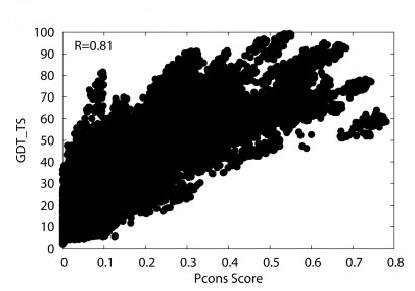
\includegraphics[scale=0.75]{pcons_correlation}
		\caption[Pcons vs GDT\_TS scattered plot]{Pcons vs GDT\_TS scattered plot.}
		\label{fig:pcons_corr}
	\end{center}
\end{figure}
Clustering methods tend to fail when the top models are far away from the cluster core or when no structural redundancy is present among the considered ensemble, determining a very sparse cluster. 
With the aim of avoiding these clustering drawbacks, QMEANclust \cite{Benkert2008ab, Benkert2008aa} uses QMEAN to select a subset of higher quality models. QMEANclust ranks models by computing the median of the distances between the current ranked model and all other models contained in the subset previously defined.\\
ModFOLDclust \cite{McGuffin2008} is a variant of the standard ModFOLD method. The global clustering score is based on the 3D-Jury \cite{Ginalski2003} method whereby each model is compared to every other model and the average structural similarity score is computed. ModFOLDclust differs from 3D-Jury, first in the use of the TMscore for pairwise comparisons and second in the server user interface allowing users to directly upload multiple models of their own choice from any source. A local MQAP version of ModFOLDclust also exists.


\cleardoublepage
